%%%%%%%%%%%%%%%%%%%%%%%%%%%%%%%%%%%%%%%%%
% Beamer Presentation
% LaTeX Template
% Version 1.0 (10/11/12)
%
% This template has been downloaded from:
% http://www.LaTeXTemplates.com
%
% License:
% CC BY-NC-SA 3.0 (http://creativecommons.org/licenses/by-nc-sa/3.0/)
%
%%%%%%%%%%%%%%%%%%%%%%%%%%%%%%%%%%%%%%%%%

%----------------------------------------------------------------------------------------
%	PACKAGES AND THEMES
%----------------------------------------------------------------------------------------

\documentclass{beamer}

\mode<presentation> {

% The Beamer class comes with a number of default slide themes
% which change the colors and layouts of slides. Below this is a list
% of all the themes, uncomment each in turn to see what they look like.

%\usetheme{default}
%\usetheme{AnnArbor}
%\usetheme{Antibes}
%\usetheme{Bergen}
%\usetheme{Berkeley}
%\usetheme{Berlin}
%\usetheme{Boadilla}
%\usetheme{CambridgeUS}
%\usetheme{Copenhagen}
%\usetheme{Darmstadt}
%\usetheme{Dresden}
%\usetheme{Frankfurt}
%\usetheme{Goettingen}
%\usetheme{Hannover}
%\usetheme{Ilmenau}
%\usetheme{JuanLesPins}
%\usetheme{Luebeck}
\usetheme{Madrid}
%\usetheme{Malmoe}
%\usetheme{Marburg}
%\usetheme{Montpellier}
%\usetheme{PaloAlto}
%\usetheme{Pittsburgh}
%\usetheme{Rochester}
%\usetheme{Singapore}
%\usetheme{Szeged}
%\usetheme{Warsaw}

% As well as themes, the Beamer class has a number of color themes
% for any slide theme. Uncomment each of these in turn to see how it
% changes the colors of your current slide theme.

%\usecolortheme{albatross}
%\usecolortheme{beaver}
%\usecolortheme{beetle}
%\usecolortheme{crane}
%\usecolortheme{dolphin}
%\usecolortheme{dove}
%\usecolortheme{fly}
%\usecolortheme{lily}
%\usecolortheme{orchid}
%\usecolortheme{rose}
%\usecolortheme{seagull}
%\usecolortheme{seahorse}
%\usecolortheme{whale}
%\usecolortheme{wolverine}

%\setbeamertemplate{footline} % To remove the footer line in all slides uncomment this line
%\setbeamertemplate{footline}[page number] % To replace the footer line in all slides with a simple slide count uncomment this line

%\setbeamertemplate{navigation symbols}{} % To remove the navigation symbols from the bottom of all slides uncomment this line
}

\usepackage{graphicx} % Allows including images
\usepackage{booktabs} % Allows the use of \toprule, \midrule and \bottomrule in tables

\usepackage{listings}
\usepackage{verbatim}

\definecolor{Brown}{cmyk}{0,0.81,1,0.60}
\definecolor{OliveGreen}{cmyk}{0.64,0,0.95,0.40}
\definecolor{CadetBlue}{cmyk}{0.62,0.57,0.23,0}
\definecolor{lightlightgray}{gray}{0.9}

\lstset{
language=bash,                  % Code langugage
basicstyle=\tiny\ttfamily,      % Code font
keywordstyle=\color{blue},      % Keywords font ('*' = uppercase)
commentstyle=\color{gray},      % Comments font
numbers=none,                           % Line nums position (e.g., left)
numberstyle=\tiny,                      % Line-numbers fonts
stepnumber=1,                           % Step between two line-numbers
numbersep=5pt,                          % How far are line-numbers from code
backgroundcolor=\color{lightlightgray}, % Choose background color
frame=single,                             % A frame around the code
tabsize=4,                              % Default tab size
captionpos=b,                           % Caption-position = bottom
breaklines=true,                        % Automatic line breaking?
breakatwhitespace=false,                % Automatic breaks only at whitespace?
showspaces=false,                       % Dont make spaces visible
showtabs=false,                         % Dont make tabls visible
columns=flexible,                       % Column format
morekeywords={find, tar, ls, bcftools},
}

% xtong's tools
% aliasis
\newcommand{\xemp}[1]{{\color{red}{\textbf{#1}}}}
\newcommand{\bs}{\boldsymbol}
\newcommand{\mean}[2]{\left\langle{#1}\right\rangle_{#2}}
\newcommand{\trb}[1]{\textrm{Tr}\left({#1}\right)}
\newcommand{\trs}[1]{\textrm{Tr}\left[{#1}\right]}
\newcommand{\invb}[1]{{\left({#1}\right)^-}}
\newcommand{\invs}[1]{{\left[{#1}\right]^-}}
\newcommand\numberthis{\addtocounter{equation}{1}\tag{\theequation}}
\renewcommand{\eqref}[1]{Eq.\,\ref{#1}}
%
% vectors and matrices
\newcommand{\va}{\boldsymbol{a}}
\newcommand{\vb}{\boldsymbol{b}}
\newcommand{\vc}{\boldsymbol{c}}
\newcommand{\vf}{\boldsymbol{f}}
\newcommand{\vg}{\boldsymbol{g}}
\newcommand{\vh}{\boldsymbol{h}}
\newcommand{\vv}{\boldsymbol{v}}
\newcommand{\vx}{\boldsymbol{x}}
\newcommand{\vu}{\boldsymbol{u}}
\newcommand{\vy}{\boldsymbol{y}}
\newcommand{\vw}{\boldsymbol{w}}
\newcommand{\vs}{\boldsymbol{s}}
% 
\newcommand{\xv}{\boldsymbol{V}}
\newcommand{\xf}{\boldsymbol{F}}
\newcommand{\xh}{\boldsymbol{H}}
\newcommand{\xk}{\boldsymbol{K}}
\newcommand{\xw}{\boldsymbol{W}}
\newcommand{\xx}{\boldsymbol{X}}
%
% random variable
\newcommand{\xu}{\boldsymbol{U}}
\newcommand{\xy}{\boldsymbol{Y}}
\newcommand{\xa}{\boldsymbol{A}}
\newcommand{\xd}{\boldsymbol{D}}
\newcommand{\xg}{\boldsymbol{G}}
% 
% with tildes
%% vectors
\newcommand{\vat}{\tilde{\vb}}
\newcommand{\vbt}{\tilde{\vb}}
\newcommand{\vct}{\tilde{\vc}}
\newcommand{\vht}{\tilde{\vh}}
\newcommand{\vvt}{\tilde{\vv}}
\newcommand{\vst}{\tilde{\vs}}
\newcommand{\vut}{\tilde{\vu}}
\newcommand{\vft}{\tilde{\vf}}
\newcommand{\xut}{\tilde{\xu}}
\newcommand{\vxt}{\tilde{\vx}}
\newcommand{\xvt}{\tilde{\xv}}
\newcommand{\xyt}{\tilde{\xy}}
%% matrices
\newcommand{\xwt}{\tilde{\xw}}
%
% with hats
\newcommand{\vhh}{\hat{\vh}}
\newcommand{\xvh}{\hat{\xv}}
\newcommand{\vvh}{\hat{\vv}}
\newcommand{\vyh}{\hat{\vy}}
\newcommand{\vxh}{\hat{\vx}}
\newcommand{\vuh}{\hat{\vu}}
\newcommand{\vfh}{\hat{\vf}}
\newcommand{\xyh}{\hat{\xy}}
\newcommand{\xxh}{\hat{\xx}}
\newcommand{\xuh}{\hat{\xu}}
%
%
% derivatives
\newcommand{\DRV}[2]{\frac{d #1}{d #2}}
\newcommand{\DRC}[3]{\DRV{#1}{#2}\DRV{#2}{#3}}
\newcommand{\PDV}[2]{\frac{\partial #1}{\partial #2}}
\newcommand{\PDC}[3]{\PDV{#1}{#2}\PDV{#2}{#3}}
%
% the diagnal matrix
\newcommand{\id}{\textrm{\textbf{I}}}
\newcommand{\im}{\textrm{\textbf{I}}}
% the vector of ones
\newcommand{\one}{\boldsymbol{1}}
% 
% xiaoran's edit
\newcommand{\xadd}[1]{\textcolor{blue}{#1}}
\newcommand{\xdel}[1]{\textcolor{red}{\sout{#1}}}
\newcommand{\xrpl}[2]{\xdel{#1}\xadd{#2}}
\newcommand{\xacc}[1]{\textcolor{ForestGreen}{#1}}
%
%
% declarations
% argument of the minimum / maximum
\DeclareMathOperator*{\argmin}{arg\,min}
\DeclareMathOperator*{\argmax}{arg\,max}

%----------------------------------------------------------------------------------------
%	TITLE PAGE
%----------------------------------------------------------------------------------------

\title[Effective HPCC]{Effective Operation on MSU HPCC} % The short title appears at the bottom of every slide, the full title is only on the title page

\author{Xiaoran Tong} % Your name
\institute[EPI Biosta, MSU] % Your institution as it will appear on the bottom of every slide, may be shorthand to save space
{
Department of Epidemiology and Biostatistics
Michigan State University \\ % Your institution for the title page
\medskip
\textit{tongxia1@msu.com} % Your email address
}
\date{\today} % Date, can be changed to a custom date

\begin{document}

\begin{frame}
\titlepage % Print the title page as the first slide
\end{frame}

\begin{frame}
\frametitle{Table of Content} % Table of contents slide, comment this block out to remove it
\tableofcontents % Throughout your presentation, if you choose to use \section{} and \subsection{} commands, these will automatically be printed on this slide as an overview of your presentation
\end{frame}

%----------------------------------------------------------------------------------------
%	PRESENTATION SLIDES
%----------------------------------------------------------------------------------------

\begin{frame}
\frametitle{The Purpose}
When wield properly, HPCC is a powerful aid for projects involving heavy computation.\\~\\

It however demands inhibiting amount of planning, setup, and post-processing. \\~\\

The main purpose of this presentation is to (not in strict order)
\begin{itemize}
\item layout the thought process of parallelism;
\item a tutorial of the HPCC helper script: \textbf{hpcwp};
\item a cookbook for for common computation tasks.
\end{itemize}

\end{frame}

%------------------------------------------------
\section{Overview} % Sections can be created in order to organize your presentation into discrete blocks, all sections and subsections are automatically printed in the table of contents as an overview of the talk
%------------------------------------------------

%\subsection{Subsection Example} % A subsection can be created just before a set of slides with a common theme to further break down your presentation into chunks

%------------------------------------------------

\begin{frame}
\frametitle{Generic Work-flow on HPCC}
For any High Performance Computation, the parallelism amount to:
\begin{block}{Step 1}
Rewrite the task as independent batches of command;
\end{block}

\begin{block}{Step 2}
Distribute the batches to many HPCC jobs then wait;
\end{block}

\begin{block}{Step 3}
Aggregate the outputs.
\end{block}
\end{frame}

%------------------------------------------------

\begin{frame}
\frametitle{Generic Work-flow on HPCC, continue}
\begin{itemize}
\item Step 2 use to be the bulk of human labor, due to hardly avoidable trail and error of PBS scripting;
\item With the help of \textbf{hpcwp} though, step 1 now stands out to be the most annoying;
\item Being careful with step 1 greatly facilitate step 2 and 3.
\end{itemize}

\end{frame}

%------------------------------------------------
\subsection{A Motivating Example}
\begin{frame}
\frametitle{A Motivating Example: Tidy up 1000 genome data}

\textbf{Description of Task:} \\
After downloading 22 \textbf{vcf.gz} from NCBI, one per autosome, we put them whin
\textbf{raw/000}, and wish to
\begin{itemize}
\item keep only SNPs with MAF \(\ge\) 0.005;
\item drop redundant information field.
\end{itemize}
Doing so would
\begin{itemize}
\item reduce the size of data;
\item speed up random access;
\item retain credible variants.
\end{itemize}
\end{frame}

%------------------------------------------------
\begin{frame}[fragile]
\frametitle{Example: Continue}
Two lines are required to process one \textbf{vcf} (one autosome):
%\begin{example}[tidy up chromosome 1]
\begin{lstlisting}
bcftools view raw/000/01.vcf.gz -i 'MAF>0.0049' -v snps | bcftools annotate -x INFO -Oz -o 01.vcf.gz
bcftools index -t 01.vcf.gz
\end{lstlisting}
%\end{example}
\begin{itemize}
\item the 2nd line depends on the first, it operates on the output file ``01.vcf.gz'';
\item thay are not interfering with other chromosomes (\textbf{\{02..22\}.vcf.gz}).
\end{itemize}
The obvious strategy is to arrange 22 batches, one for each autosome, two lines per batch.
\end{frame}

%------------------------------------------------

\begin{frame}[fragile]
\frametitle{Example: Continue}
\textbf{Step 1: Rewrite the task as independent batches of command} \\
suppose we wrote them in "\verb|src/tidy.sh|", under the present working directory.
\begin{example}[22 batches of command to tidy up 22 autosomes]
\begin{lstlisting}
# ------ within src/tidy.sh ------ #
bcftools view raw/000/01.vcf.gz -i 'MAF>0.0049' -v snps | bcftools annotate -x INFO -Oz -o 01.vcf.gz
bcftools index -t 01.vcf.gz
bcftools view raw/000/02.vcf.gz -i 'MAF>0.0049' -v snps | bcftools annotate -x INFO -Oz -o 02.vcf.gz
bcftools index -t 02.vcf.gz
        ...      ...
bcftools view raw/000/22.vcf.gz -i 'MAF>0.0049' -v snps | bcftools annotate -x INFO -Oz -o 22.vcf.gz
bcftools index -t 22.vcf.gz
# ------ end of src/tidy.sh ------ #
\end{lstlisting}
\end{example}
The principle is, the batches of command must accomplish the same when executed sequentially, given an
infinite time budget.
\end{frame}

%------------------------------------------------

\begin{frame}[fragile]
\frametitle{Example: A look around before Step 2}
\begin{figure}
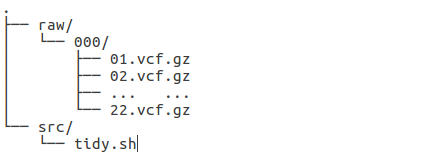
\includegraphics[width=0.7\linewidth]{img/step1}
\end{figure}
\begin{itemize}
\item the top \textbf{"."} points to the present working directory (\textbf{PWD})
\item "raw" and "src" are visible under PWD
\item items further down the tree must be referred via full name, e.g.:
  \begin{itemize}
  \item raw/000/01.vcf.gz
  \item src/tidy.sh
  \end{itemize}
\end{itemize}

\end{frame}

%------------------------------------------------

\begin{frame}[fragile]
\textbf{Step 2: dispatch the batches to HPCC jobs} \\
Dispatch the 22 batches to 22 jobs.
the downloaded autosomes are located in \textbf{raw/000}, we plan to place the output in \textbf{raw/100};
\begin{example}[22 batches dispatched to 22 jobs]
\begin{lstlisting}
hpcwp src/tidy.sh -d raw/100 -q2 --ln raw # prepare the jobs
cd raw/100                                # goto job home / output
./sub.sh                                  # submit the jobs
# grep a cut of tee and wait, use 'qstat -u <ID> to monitor the HPCC jobs.
\end{lstlisting}
\end{example}
\begin{itemize}
\item \textbf{hpcwp} scans 44 lines in "\textbf{src/tidy.sh}" top to bottom;
\item \textbf{raw/100} is the \textbf{job home}, specified by the \textbf{-d} option;
  \begin{itemize}
  \item letting the \textbf{job home} be the same with planed output directory is a common practice.
  \item the \textbf{jobs} will be put under "\textbf{raw/100/pbs}"
  \end{itemize}
\item \texttt{-q2} set the queue size to \textbf{2}, hence $44 \div 2 = 22$ batches(*)
\end{itemize}
\end{frame}

%------------------------------------------------
\begin{frame}
\frametitle{More Explanation:}
\begin{itemize}
\item {\color{red}\texttt{--ln raw}} creates a symbolic link within the job home
  '\textbf{raw/100}' pointing to \textbf{raw}, only then will HPCC be
  able to to 'see' the folder 'raw' when it gose inside of the job
  home.
\item {\color{red}\texttt{cd raw/100}} change the present working
  directory to the job home, where we call
  {\color{red}\texttt{./sub.sh}} to submit them, and wait for them to
  finish;
\item use \texttt{qstat -u <MSU NetID>} to monitor the execution.
\end{itemize}
\end{frame}
% ------------------------------------------------
\begin{frame}
  \frametitle{Step 2: job praperation}
  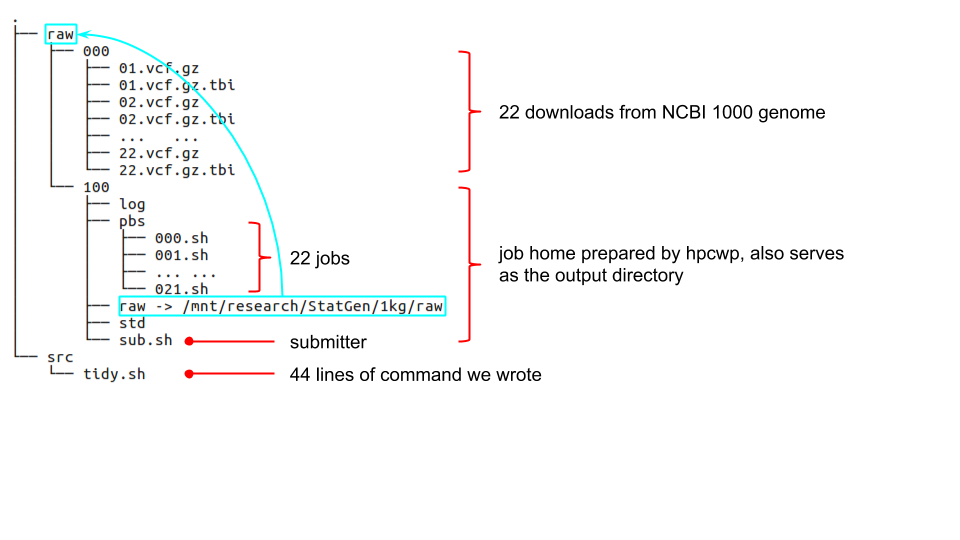
\includegraphics[width=1.0\linewidth]{img/step_2_a}
\end{frame}
% ------------------------------------------------
\begin{frame}
  \frametitle{Step 2: job praperation, continue}
  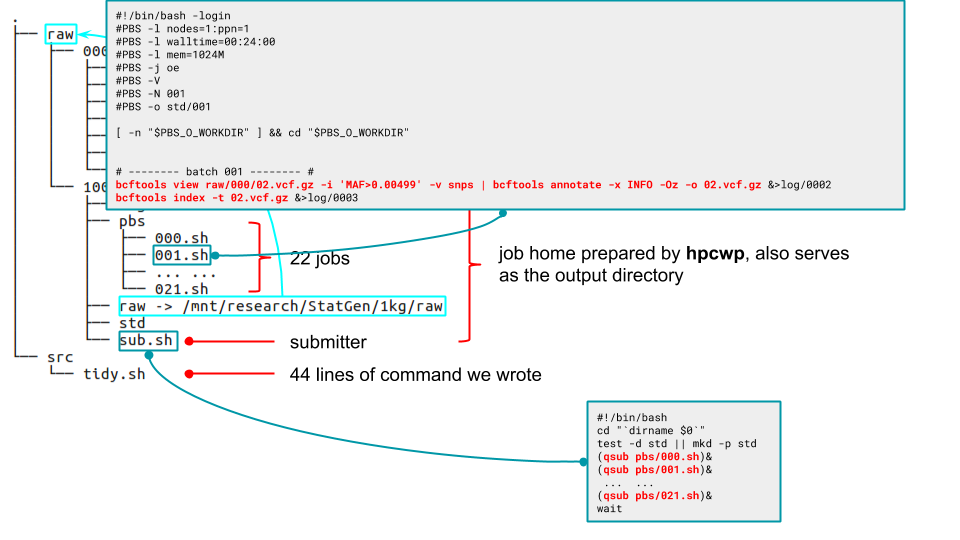
\includegraphics[width=1.0\linewidth]{img/step_2_b}
\end{frame}
% ------------------------------------------------
\begin{frame}
  \frametitle{step 2: job monitoring}
  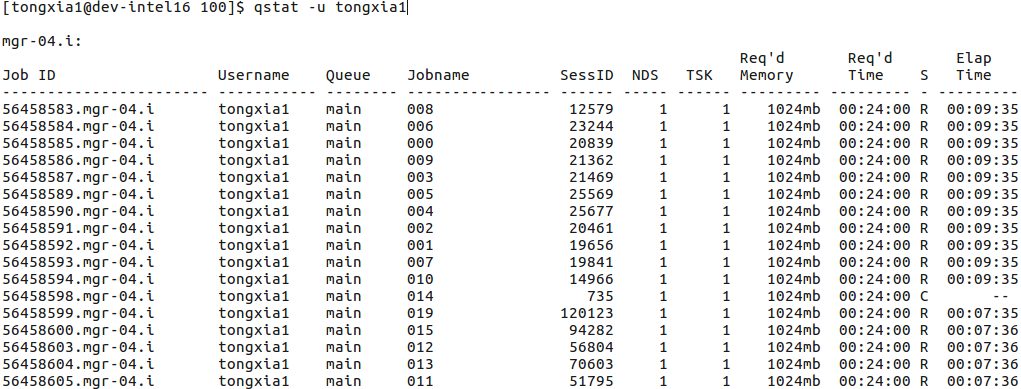
\includegraphics[width=1.0\linewidth]{img/step_2_c}
\end{frame}
% ------------------------------------------------
\begin{frame}
  \frametitle{Step 2: finish}
  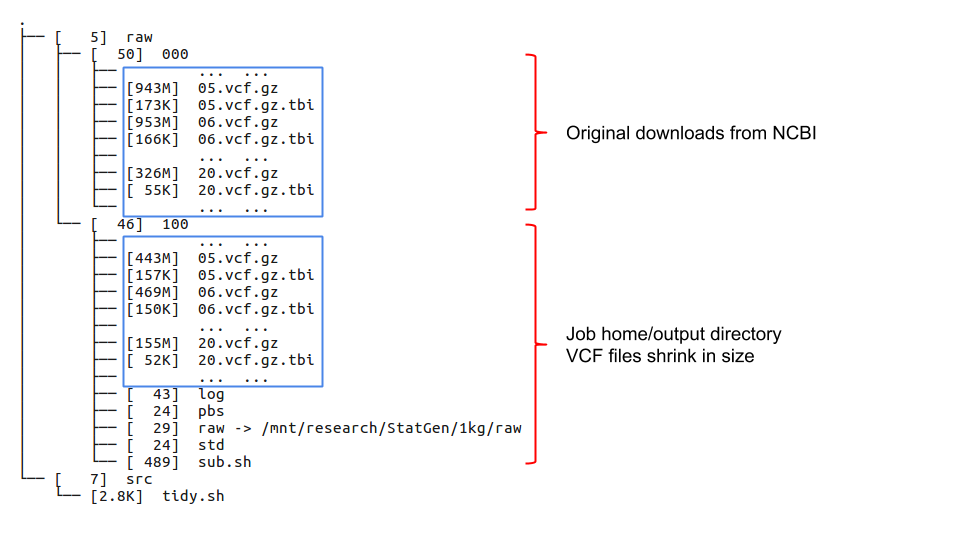
\includegraphics[width=1.0\linewidth]{img/step_2_d}
\end{frame}
%------------------------------------------------

\begin{frame}
\textbf{Step 3: aggregate output}
For this particular data clean up operation, there is no need to collect output. For most scientific
computation (e.g., simulation), this is necessary.
\end{frame}

%------------------------------------------------
\section{hpcwp -- The HPCC Wrapper}
\begin{frame}
  \frametitle{The HPCC Wrapper}
  The hpcwp script can do more:
  \begin{itemize}
  \item 
  \end{itemize}
\end{frame}
%------------------------------------------------
\section{Tested Practices}
\subsection{covernt scripts to commands (stub)}
\begin{frame}
  \frametitle{covernt scripts to commands (stub)}
  Scripts are usually compsed and tested interactively (i.e., under a
  programing enviroment like RStudio), but itself is not sutible for
  parallel computation; \\
  it must be able to execute non-interactively; \\
  \textbf{quick workaround}
  \begin{itemize}
  \item R: Rscript -e 'source("script.R"); fun(...)'
  \item Python3.x: python3 -c `import fun from script; fun(...)'
  \end{itemize}
  \textbf{covent scripts to commands}
  \begin{itemize}
  \item use special header ``!\#Rscript'' or ``!\#python3''
  \item \texttt{chmod +x} (linux only)
    \begin{itemize}
    \item \textbf{hpcwp} is itself a python script turned command.
    \end{itemize}
  \end{itemize}
\end{frame}
%------------------------------------------------
\subsection{compose series of commands (stub)}
\begin{frame}
  \frametitle{compose series of commands}
  \begin{itemize}
  \item in the motivation example, writing 24 commands into
    ``tidy.sh'' was tedious but not impossible
  \item in many project however, the number of commands is impractical for manual typing:
    \begin{itemize}
    \item write Freesurfer importation commands for 808 ADNI subjects;
    \item another 808 for cortex reconstruction;
    \item 100 simulations to compare 3 metods over 4 sample sizes, 1200 in total;
    \end{itemize}
  \item automated command writing:
    \begin{itemize}
    \item use excel
    \item use \xemp{R}: \textbf{expand.grid}, \textbf{paste}, and
      \textbf{sprintf}
    \item use Python generator/iterator and string.format
    \item use GNU script
    \end{itemize}
  \end{itemize}
\end{frame}
%------------------------------------------------
\subsection{aggregate outputs (stub)}
\begin{frame}
  \frametitle{aggregate outputs}
  We try everything to minimize human labor
  \begin{itemize}
  \item Using R:
    \begin{itemize}
    \item \xemp{dir} to enumerate output filenames;
    \item \xemp{read.\{talbe, delim, csv\}} + \xemp{lapply} to read all outputs
      as R \xemp{data.frame}, and put into an R \xemp{list};
    \item \xemp{do.call} + \xemp{cbind} to concatenate all data frames;
    \end{itemize}
  \end{itemize}
\end{frame}
%------------------------------------------------
\begin{frame}
\Huge{\centerline{The End}}
\end{frame}
%----------------------------------------------------------------------------------------

\end{document} 